%\documentclass[letterpaper, 10 pt, conference]{ieeeconf}  % Comment this line out
                                                          % if you need a4paper
\documentclass[a4paper, 10pt, conference]{ieeeconf}      % Use this line for a4
\usepackage{FG2018}
%\FGfinalcopy % *** Uncomment this line for the final submission
\IEEEoverridecommandlockouts                              % This command is only
                                                          % needed if you want to
                                                          % use the \thanks command
\overrideIEEEmargins
% See the \addtolength command later in the file to balance the column lengths
% on the last page of the document
% The following packages can be found on http:\\www.ctan.org
\usepackage{graphics} % for pdf, bitmapped graphics files
\usepackage{multicol}
\usepackage{lipsum}
\usepackage{tikz}
\usepackage{epsfig} % for postscript graphics files
\usepackage{mathptmx} % assumes new font selection scheme installed
\usepackage{times} % assumes new font selection scheme installed
\usepackage{amsmath} % assumes amsmath package installed
\usepackage{amssymb}  % assumes amsmath package installed
\usepackage{algorithm,algorithmic}
\usepackage{caption}
\usepackage{multirow}
\usepackage{verbatim}
\usepackage{stfloats}
\usetikzlibrary{shapes,arrows,chains}
\usepackage{xcolor}
%\usepackage{cite}
\graphicspath{{../pdf/}{../jpeg/}}
\DeclareGraphicsExtensions{.pdf,.jpeg,.png}
\def\FGPaperID{****} % *** Enter the FG 2018 Paper ID here

\title{\LARGE \bf
An Efficient Method Utilizing Temporal Correlationship for Real-time Face Alignment
}

%use this in case of a single affiliation
%\author{\parbox{16cm}{\centering
%    {\large Huibert Kwakernaak}\\
%    {\normalsize
%    Faculty of Electrical Engineering, Mathematics and Computer Science, University of Twente, Enschede, The Netherlands\\}}
%    \thanks{This work was not supported by any organization.}% <-this % stops a space
%}

%use this in case of several affiliations


\begin{document}

\ifFGfinal
\thispagestyle{empty}
\pagestyle{empty}
\else
\author{\parbox{16cm}
	{\centering
		{
		\large Mengran Lin$^1$ and Xinliang Wang$^1$\\
				 Jingcong Chen$^1$ and Cheng Yi$^1$\\
				 Chi Xi$^1$ and Bin Li$^1$
		}\\
		{\normalsize
			%$^1$ Faculty of Electrical Engineering, Mathematics and Computer Science, University of Twente, Enschede, The Netherlands\\
             $^1$Chengdu R\&D Center, Tencent Technology Co.,Ltd, China
		}
	}
	\thanks{This work was not supported by any organization}% <-this % stops a space
}
\pagestyle{plain}
\fi
\maketitle
%%%%%%%%%%%%%%%%%%%%%%%%%%%%%%%%%%%%%%%%%%%%%%%%%%%%%%%%%%%%%%%%%%%%%%%%%%%%%%%%
\begin{abstract}
This paper addresses the problem of real-time face alignment.
Usually, this problem is tackled by alignment in each individual frame.
However, it suffers from limited performance involving temporal continuity, which is concretely reflected in smooth alignments.
The underlying reason is that the temporal correlationship between shapes of adjacent frames doesn't be utilized.
Therefore, we propose a real-time face alignment technique utilizing the temporal correlationship, namely shape residuals between
consecutive frames in this paper.
Specifically, we postulate that the shape residuals have a sparse pattern in some domain.
Under the hypothesis, They can be explictly depicted by an offline model trained within compressive sensing framework.
Once the residuals are recovered, we can obtain an alignment of each current frame by adding them to shape of the corresponding last frame.
Otherwise, to avoid shape drift or loss during the real-time face alignment, a reboot mechanism is adopted to effectively align
a current shape.
Experimental results demonstrate the superior performance of our approach compared with the state-of-the-arts in terms of smoothness
and working efficiency.
\end{abstract}
%%%%%%%%%%%%%%%%%%%%%%%%%%%%%%%%%%%%%%%%%%%%%%%%%%%%%%%%%%%%%%%%%%%%%%%%%%%%%%%%
\section{INTRODUCTION}
Static face alignment, namely performing face alignment in a static images in large-scale and unconstrained conditions has been a most
studied topic within the computer vision community during the last decades. As accurate localization of fiducials is a vital
prerequisite task for variety of applications, e.g., face recognition \cite{wagner2012toward}, 3D face reconstruction
\cite{roth2015unconstrained,roth2016adaptive}, face de-identification \cite{jourabloo2015attribute} and expression analysis
\cite{guo2016dynamic,hu2014robust,vogler2007best}. 

% methods in static face alignment
The existing static face alignment approaches mainly start the alignment process from the mean facial shape \cite{ren2014face}, and deform the shape constrained by 
offline-trained facial deformable parameterized models (FDPMs) to minimize the shape residual by gradient descend optimization. 
Active Shape Model (ASM) based approaches \cite{tecootes1994active} and Active Appearance Models (AAM) based approaches 
\cite{edwards1998interpreting,matthews2004active} are typical representative subject to this category. Recently, regression based approaches
\cite{valstar2010facial,dollar2010cascaded,cao2014face,xiong2013supervised,tzimiropoulos2015project}, which attempt to infer a face shape 
through a discriminative regression function by directly mapping textual features to shape, have been proposed with excellent performance.
Moreover, the tree based cascade regression approaches \cite{ren2014face,kazemi2014one,cao2014face,burgos2013robust} provide a super 
real-time performance.
Although the methods of static face alignment have shown great success in standard benchmark datasets \cite{sagonas2013300} with respect to
the efficiency,
many of them suffer from significant performance degradation especially in real-world scenarios under wild conditions
\cite{shen2015first,peng2016sequential}.
These methods are not appropriate for real-time face alignment, for
they usually align each frame independently from a stable initial shape, e.g., a mean face in a tracking-by-detection manner by various facial 
landmark detectors \cite{decarlo2000optical} Therefore, this manner does not utilize the temporal correlationship between consecutive frames,
and results in a un-smooth fitting. Otherwise, offline-trained static facial deformable models (FDMs) can not express some large shape residual precisely.
Therefore, real-time face alignment, namely fitting facial landmarks on
consecutive frames, is still very challenging and there is only a few published work in this direction. Therefore, this is a clear
research gap that needs to be addressed, which is exactly the focus of this work.

To exploit the temporal correlationship, the existing approaches for real-time face alignment usually adopt a tracking manner 
\cite{vogler2007best,wettum2017facial}, in which
the location of facial landmarks in preceding frames can be used to find the facial landmarks in the current frame.
These approaches take advantage of location of facial landmarks in the last frame or multiple nearly-optimum initial estimated results to
find the facial landmarks in a current frame by minimizing shape residual. It exploits the fact that the various changes of face shape over time
are smooth in videos. Then, the offline trained FDMs can capture the shape residual if the previous landmarks were detected with acceptable accuracy,
which make the initial estimated shape be close enough to the current landmarks. Hence, tracking based approaches are more likely to produce highly
accurate, illumination-change-robust and partial-occlusion-robust fitting results than the aforementioned static approaches.
% incremental methods
As described above, the tracking based approaches still employ the trained FDMs 
built offline using a set of static annotated facial images, which does not include the subject being tracked \cite{sanchez2016cascaded}
to recover the shape residual from a close initializations. This may inevitably result in shape drift when starting from poor initial estimations
for the reason that the offline FDMs are weak in expressing shape residual. Hence how to enlarge expression to shape residual for offline FDMs
is an important problem. Therefore, incremental learning based approaches
\cite{sanchez2016cascaded,peng2016sequential,sung2009adaptive,asthana2014incremental,peng2015piefa}
are proposed to address the problem in an online manner, which improve the generic offline FDMs into a person-specific one.

In summarize, the existed approaches for real-time face alignment are respectively:
\begin{itemize}
    \item Static face alignment based approaches, as illustrated in Figure \ref{fig:niubility}(a), fit the current shapes, represented by red points, from mean shape,
          represents by green point individually.
      \item Tracking based approaches, as illustrated in Figure \ref{fig:niubility}(b), fit the current shape, represented by red point, by searching the inner green
          region which is smaller than the outer one, last frame shape may be in.
    \item Incremental learning based approaches, as illustrated in Figure \ref{fig:niubility}(c), fit the current shape from a bigger searching region, represented by
          green color, relative to that of Figure \ref{fig:niubility}(b).
\end{itemize}
However, incremental methods are nearly real-time \cite{sanchez2016cascaded}, since incremental learning is costly, which severely impedes
their applications on tasks need high real-time performance. Therefore, how to improve the offline FDMs with a better real-time performance is our
concern.
\begin{figure}
        \centering
        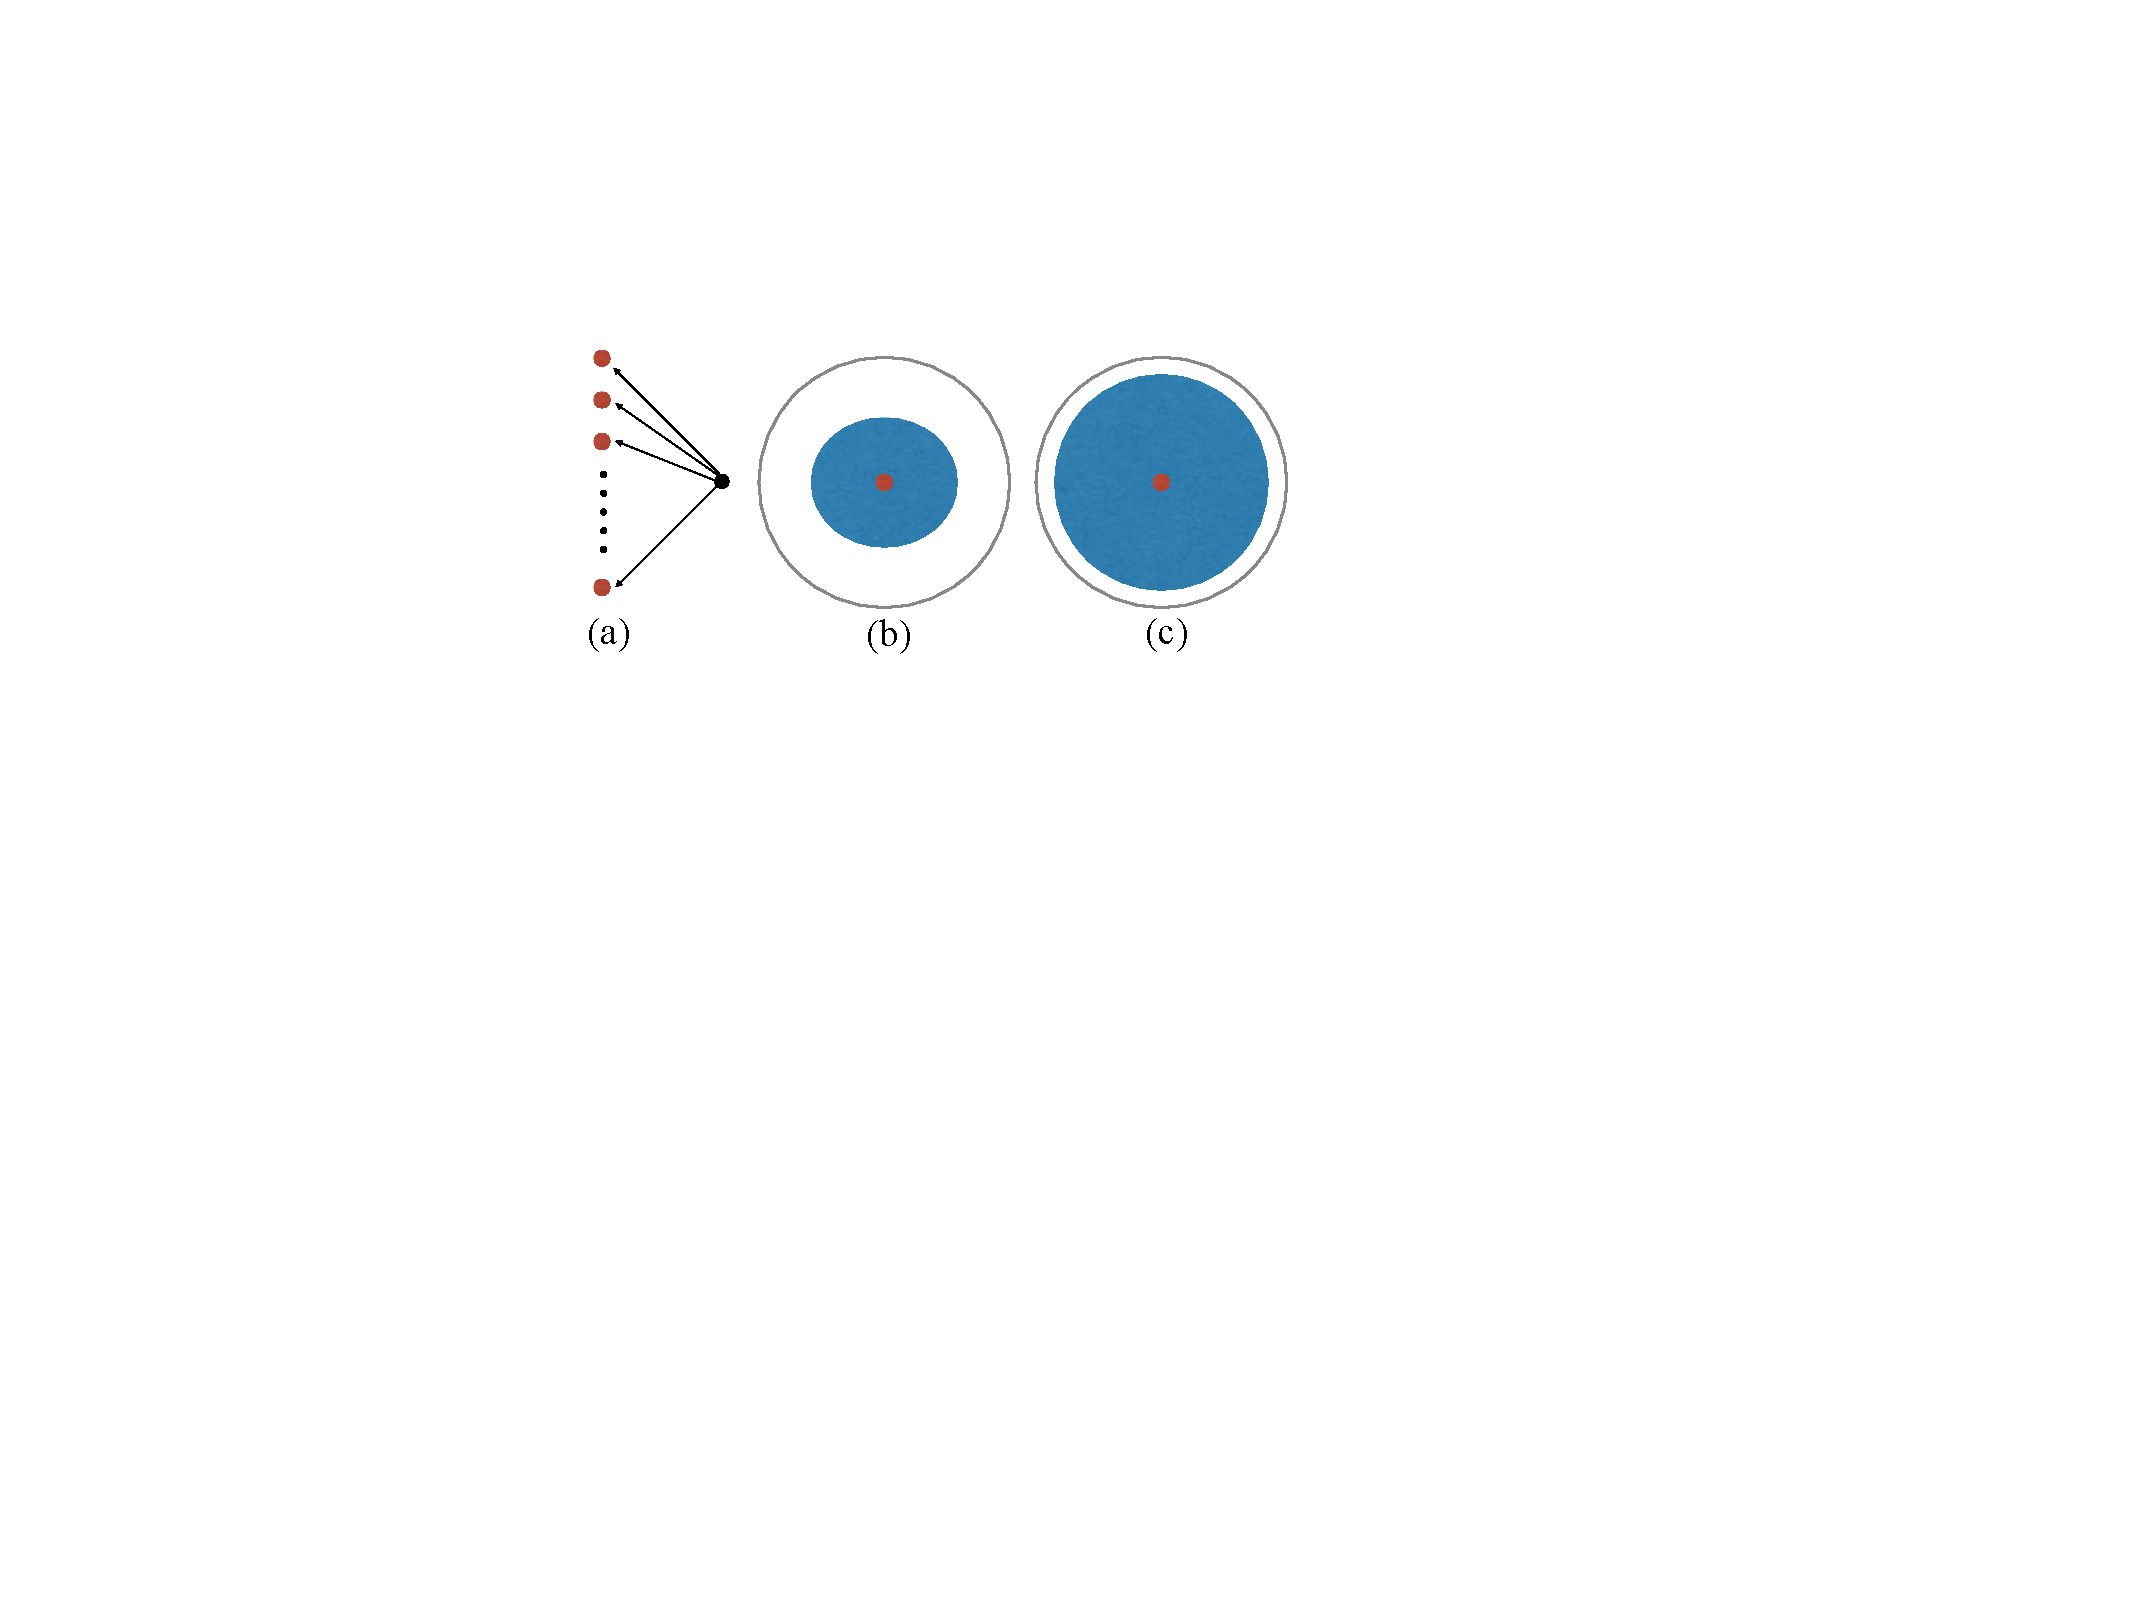
\includegraphics[width=0.45\textwidth]{niubility.pdf}% 1\linewidth  
        \caption{
        Summary of the existed approaches for real-time face alignment. The red points represent the face shapes of current frames, the black point
        represents the mean face shape. The blue region, in which the face shapes of last frames may occur, indicates the ability that
        offline FDMs express the corresponding shape residuals. (a) represents the static face alignment based approaches. (b) represents the tracking
        based approaches, and the offline FDMs of these approaches can only tackle a part of the whole search region, in which the face shapes of
        last frames may occur. (c) represents the incremental learning based approaches and our proposed strategy, they all can enlarge offline FDM's in (b)
        expression to shape residuals. What the difference is, our strategy achieves that by an offline training task.
        }
        \label{fig:niubility}
\end{figure}
\subsection{Compressive sensing based approach for real-time face alignment}
% our propposed method based on compressed sensing
%In this paper, we devote to  address aforementioned issues, we propose a novel approach based
This problem can be addressed in an offline manner compared to incremental learning based approaches. Specifically, we hope to enlarge expression to
shape residual for offline FDMs during an offline training task, as illustrated in Figure \ref{fig:niubility}(c), which is same with the incremental learning based 
approaches but the enlarging manner of our proposed approach is offline. Motivated by the face recognition application \cite{wright2009robust},
which proposes a general classification algorithm for object recognition based on sparse representation,
we postulate that the shape residuals have a sparse pattern in some domain. Under the hypothesis,
we propose a novel approach based on sparse representation to train an offline FDM which constructed
from simulated sequential training data to perform real-time face alignment. To generate the simulated sequential training data,
we randomly synthesis multiple shapes of last frame around the current truly shape. The offline FDM which captures residual between adjacent
shapes is then achieved using sparse representation. During the fitting process, we start from the estimated result and inference the current
shape through the trained offline FDM, while a reboot mechanism is adopted to alleviate model drifting. The major contributions of this paper are: 
\begin{itemize}
	\item To the best of our knowledge, this is the first work to perform real-time face alignment by an offline person-specific FDM.
	\item The proposed training strategy is radically different from existing methods with respect to the sparse representation.
	\item The proposed offline FDM is well designed for learning the temporal correlationship, and guarantees robust and real-time face alignment on
           the fly.
\end{itemize}
By conducting extensive experiments on multiple unconstrained databases, we show that our approach has significant real-time performance
smoothment improvement compared with state- of-the-art, while constant computational cost w.r.t. both CPU time and memory usage is guaranteed.
These merits make our approach very suitable for real-time and large scale applications.
\section{Method}
This section briefly reviews the theory of compressive sensing and sparse representation,
and formulates our offline FDM under compressive sensing framework for real-time face alignment. Then,
the details of training compressive sensing based offline FDM and fitting facial shape utilizing trained FDM are described.
\subsection{Compressive Sensing and Sparse Representation}
We use $x\in R^m$ to represent as a vector, the 1D dense signal to be reconstructed, let D : $ R^n\rightarrow R^m$ represents sparse transform,
which gives a sparse representation (mostly zero), $y\in R^n$, of $x$.
Compressive sensing reveals that the dense signal $ x $ can be recovered if it is sparse under $D$. We formulate it as:
\begin{equation}
    \min_{\alpha} \| \alpha \|_{0} \quad \quad \text{s.t.}\quad x = D(\alpha)
\end{equation}
Here $\| \cdot \|_{0}$ denotes $l^0$-norm, which counts the number of nonzero entries in a vector, $\alpha \in R^n$ is sparse representation of $x$.
Usually, $D$ can be pre-defined or data-driven sparse transform. The problem of finding the sparsest solution of an under-determined system
of linear equations is NP-hard. However, there are greedy algorithms to solve this problem such as orthogonal matching pursuit (OMP)
\cite{perakis20133d}. Alternatively, the $l_0$ quasi norm is replaced with its convex relaxation, the $l_1$ norm, at which the problem
can be solved via linear programming.
% this section formulate the FDM by CS
\subsection{Compressive Sensing Based Offline FDM (CS-OFDM)}
At the beginning, we introduce some notation.
Let $I$ be a face image and $X$ be its truth shape. For temporal scenario, we refer to $I_t$ as the $t$ frame image and the same to $X_t$.
The recovery of shape residuals under the compressed sensing framework aims to solve the following optimization problem:
Inspired by the theory of compressive sensing. Specifically, we presume the shape residuals have a sparse pattern in the domain concerned with
face appearance, which could reflect the motion of face. Due to this hypothesis, our problem can be formulated under compressive sensing framework.
\begin{equation}
\label{e:CS0}
	\begin{split}
        &\min_{\Gamma} \sum_{t}{\|(X_{t} - X_{t-1}) - W\{D(I_{t},X_{t-1})\}\|_2^2}\\
        &\quad\quad \text{s.t.}\quad \|D(I_{t},X_{t-1})\|_0 \leq T_0 \quad \forall t
	\end{split}
\end{equation}
The term $(X_{t} - X_{t-1})$ in Equation (\ref{e:CS0}) represents the shape residuals to be recovered. Function $D(\cdot,\cdot)$
represents the sparse transform, which is our CS-OFDM. $D(I_t,X_{t-1})$ is the sparse representation of $(X_{t} - X_{t-1})$, and $W\{D(I_{t},X_{t-1})\}$ is the estimation
of $(X_{t} - X_{t-1})$. The $l_0$ quasi norm is used to encode the sparsity of the shape residual, and $T_0$ is the
required sparsity level. $\Gamma$ is used to denote the set of sparse representations of all shape residuals. This learning formulation minimizes
the total fitting error of all shape residuals with respect to the sparse transform, $D(\cdot,\cdot)$, subject to sparsity constraints.
Our sparse transform, $D(\cdot,\cdot)$, based on face appearance conducts sparse representation. In other words, we can index the sparse
representation of the shape residuals by appearance of current frame and the last frame shape. Once that is indexed, the shape residuals can be 
estimated, and then, the estimation to current frame shape can be confirmed.

% modify this section, which mainly talk about training
\subsection{Training of Compressive Sensing Based Offline FDM}
In this section, we give the explicit details of the training process, in which we obtain the data-driven CS-OFDM. In this paper, our CS-OFDM is
trained with the static annotated dataset, $A:\{(I_0,X_0), (I_1,X_1), ... , (I_{n-1},X_{n-1})\}$. Therefore, we should construct the sequential
training samples. At first, we introduce some notation and re-formulate our problem. Then, how to simulate sequential training samples will be
introduced. At last, we will depict the training details of our proposed CS-OFDM.

Let $S$ be the set of training samples, in which the samples, $S^j$, concerned with image $I_j$, namely current frame image, will be 
$S^j:\{ (I_j,X_{c,j},\hat{X}_{l,j}^0),(I_j,X_{c,j},\hat{X}_{l,j}^1), \dots ,(I_j,X_{c,j},\hat{X}_{l,j}^{n-1}) \}$.
$c$ represents the current frame, $l$ represents the last frame. Hence, $X_{c,j}$ is the truly shape of the current frame
and $\hat{X}_{l,j}^i$ is the $i$th simulated last frame shape. Then, Equation (\ref{e:CS0}) can be re-formulated as:
\begin{equation}
\label{e:CS1}
	\begin{split}
        &\min_{\Gamma} \sum_{i,j}{\|(X_{c,j} - \hat{X}^i_{l,j}) - W\{D(I_j,\hat{X}^i_{l,j})\}\|_2^2}\\
        &\quad\quad \text{s.t.}\quad \|D(I_j,\hat{X}^i_{l,j})\|_0 \leq T_0 \quad \forall i,j
	\end{split}
\end{equation}
% Therefore, we regraded the pixel intensities relative to the last facial shape as image features.
% Then, we trained the CS-OFDM by the simulated sequential training samples
% At last, the trained CS-OFDM is utilized to perform fitting the shape residual.
\subsubsection{Sequential training samples simulation}
To generate the simulated sequential training samples, we randomly synthesis multiple last frame shapes around each annotated shape,
which is regarded as current frame shape.
The last facial shapes around the current one and the residual may occur in the scale, rotation and translation.
The theory of compressive sensing implies that the precise choice of feature space is no longer critical:
Even random features contain enough information to reflect the truth situation.
Therefore, we can randomly sample multiple shapes around the current
facial shape with various scale, rotation and translation settings.
Let $s$ denote scale random variable, $r$ denote rotation random variable, $t$ denote translation random variable.
We suppose that the population distributions of these variables all are known to be normal, with mean $\mu_1$, $ \mu_2$, and $\mu_3$,
and variance $\sigma_1^2$, $\sigma_2^2$, and $\sigma_3^2$, that are,
$s\sim N(\mu_1,\sigma_1)$, $r ~ \sim N(\mu_2, \sigma_2)$,
and $t \sim N(\mu_3,\sigma_3)$, in which $\mu_1$ is the scale of $X_{c,:}$, $\mu_2$ is the rotation of $X_{c,:}$,
and $\mu_3$ is the translation of $X_{c,:}$.
We obtain $\{s_1, s_2, ... , s_n\}$, $\{r_1, r_2, ... , r_n\}$, and $\{t_1, t_2, ... , t_n\}$ at the normal pattern. 
Once these parameters of deformation are sampled, we can apply them to $X_{c,\cdot}$ and obtain $n$ simulated last facial shapes,
$\{\hat{X}^0_{l,\cdot}, \hat{X}^1_{l,\cdot}, ... , \hat{X}^{n-1}_{l,\cdot}\}$.
\subsubsection{Training CS-OFDM}
% generate the random forest.
We alternate between learning the sparse transform and sparse representations, and estimating the facial shape residual
in a multi-stage coarse-to-fine manner to better fit the shape residuals. Otherwise,
to obtain super real-time performance, we construct the sparse transform using the tree structure which has effective search.
Specifically, after training stage $d$ with training set $S_d$ and before creating the regression tree based sparse transform (RTST)
in stage $d+1$, we use the RTSTs, trained forest, to
estimate the shape residual of each sample $s_i \in S_d$. Then, $S_{d+1}$ is updated and is utilised to train the RTST in stage $d+1$. The forest
is further grown in order to minimise the sum of square error loss as described in Equation (\ref{e:CS1}).
The alternative is repeated until a series of RTSTs are learnt, which will give a sufficient level of accuracy. The RTSTs constitute our
final CS-OFDM. In the next part, we will introduce that how to learn the $i$th RTST.

The regression tree based sparse transform is trained using a standard regression random forest \cite{breiman2001random} with the 
aforementioned dataset $S_j$ in stages, where each stage corresponds to a non-leaf vertex in the $M$. Starting with the root vertex, $i = 0$,
of $M$ we grow the tree with the objective of separating the samples in $S_j$ into two cohesive sub-regions, $S(j,l)$ and $S(j,r)$, which correspond
to the vertices $l(i)$ and $r(i)$, which are the children of the root node. The process is then repeated recursively on each split of the data,
$S(j,l)$ and $S(j,r)$, until the information gain falls below a threshold. Once the RTST is constructed, for any leaf node, $k$,
stores a 2D offset vector, $C_k$, that averages the samples, $L_k$, in the leaf, namely:
\begin{equation}
    \label{e:barwq8}
    C_k =  P_k^T * L_k
\end{equation}
where, $n_k$ is the number of samples in the $k$th leaf node, then $P_k$ is, $[\frac{1}{n_k},\frac{1}{n_k},\cdot,\frac{1}{n_k}]^T \in R^{n_k}$.

This separation is achieved by using the pixel-difference appearance feature (PDAF). At each node, we randomly generate splitting candidates,
$\Phi = \{(f_i,\tau_i)\}$, consisting of a PDF function,$f_i$ and threshold, $\tau_i$, and greedily pick the candidate $(f_j,\tau_j)$
from $\Phi$ that gives rise to maximum variance reduction.

For any two face images, $I_i$, $I_j$, with any estimated shapes, $\hat{X}_i$, $\hat{X}_j$, we would like to index the same positions of pixels 
in $I_i$ relative to its shape, $\hat{X}_i$, as the positions in $I_j$ to its shape, $\hat{X}_j$. To achieve this, each image can be warped to 
the mean shape based on the current estimated shape before extracting the features \cite{kazemi2014one}. Otherwise, a very sparse representation
of the image is much more efficient to warp the location of points as opposed to the whole image as suggested by \cite{cao2014face,kazemi2014one}.

%solve the sparse representation using the tree constructed
Once the RTST is learnt, sparse representation can be performed on each facial shape residual.
Specifically, sparse representation, $D(I_j,\hat{X}^i_{l,j})$, of each image $I_j$ with the last facial shape $\hat{X}^i_{l,j}$
can be solved based on the leaf, $k$, that shape residual reaches, i.e., the leaf at the end of the path in the tree the shape residual will follow,
and for each node $\mu$ along this path we say that arrives at $\mu$. Figure \ref{fig:sparse_representation} illustrates the process of performing 
the sparse coding, and the sparse representation can be formulated as:
\begin{figure}
        \centering
        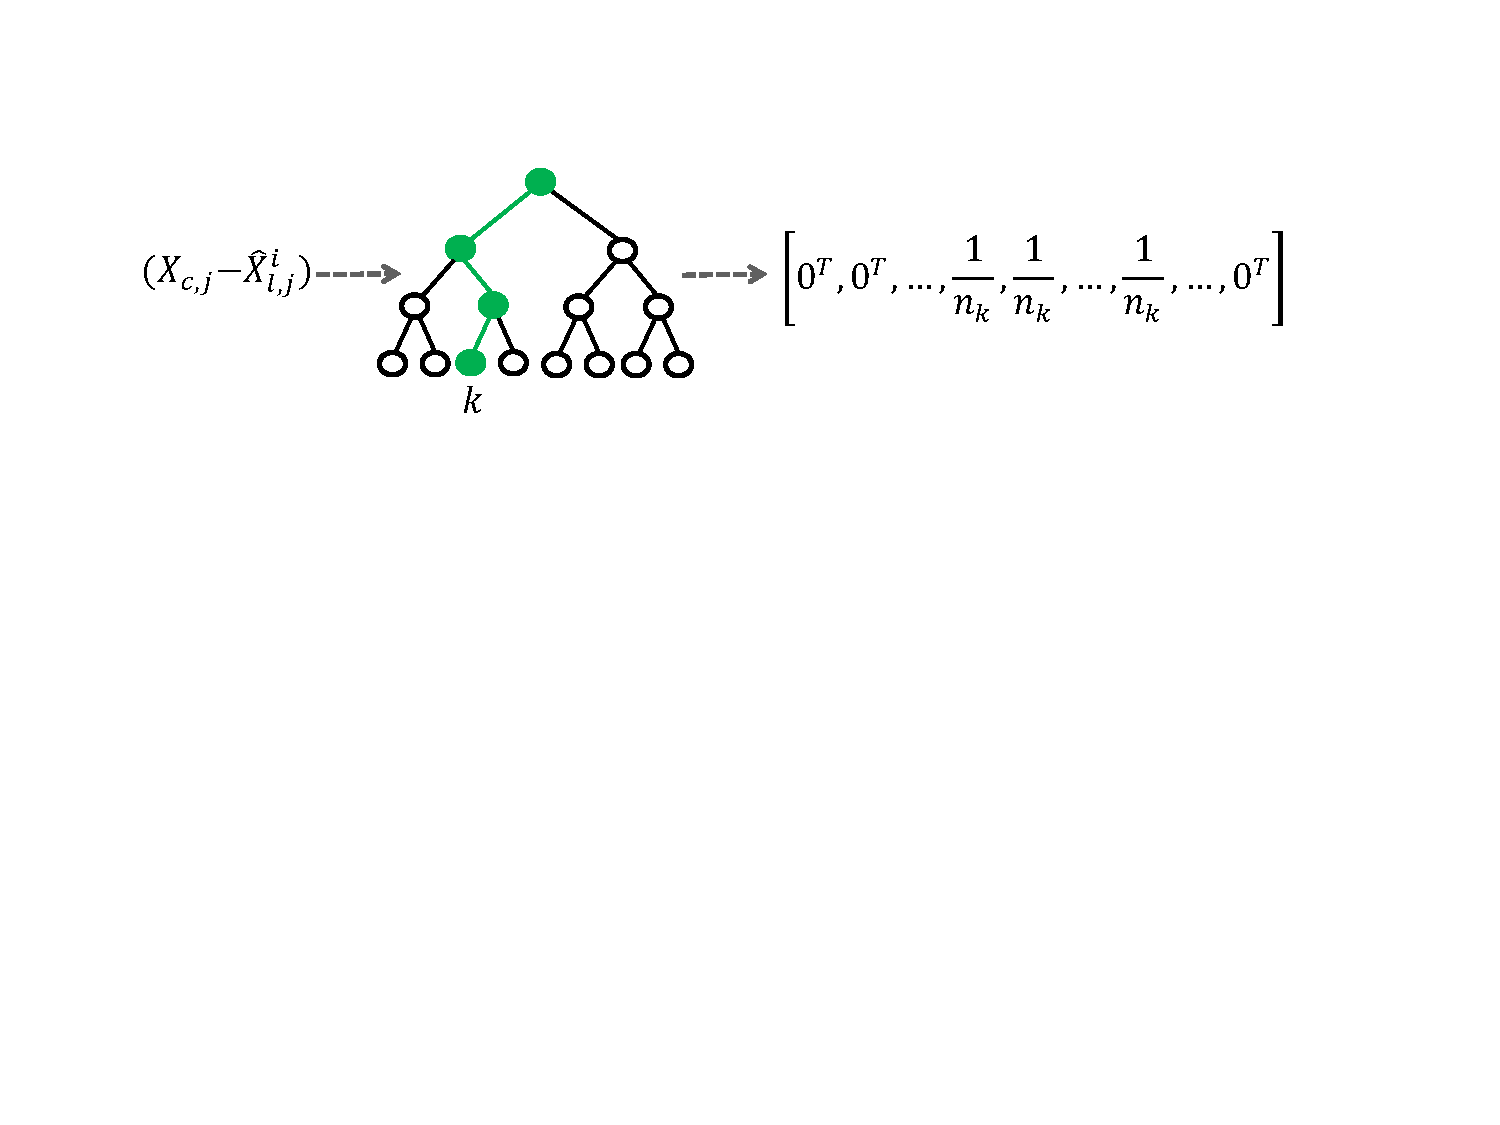
\includegraphics[width=0.48\textwidth]{sparse_representation.pdf}% 1\linewidth  
        \caption{
        Sparse coding. The regression tree based sparse transform
        encodes the shape residual into a sparse representation.
        }
        \label{fig:sparse_representation}
\end{figure}
\begin{figure}
        \centering
        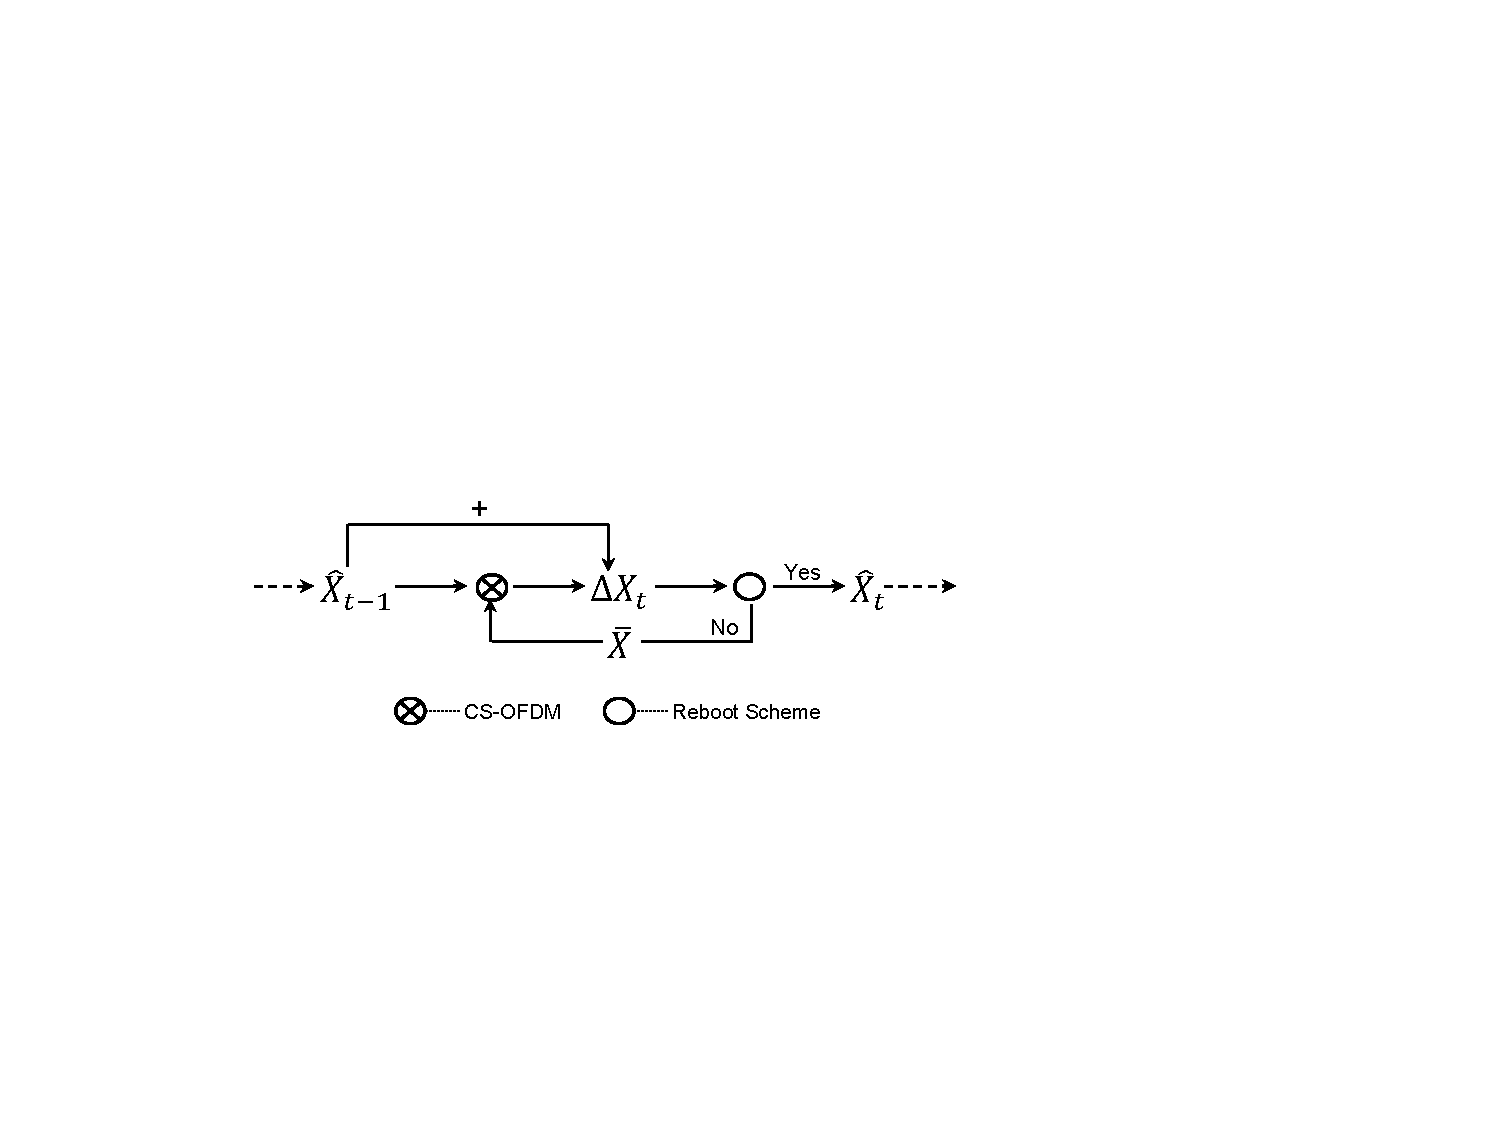
\includegraphics[width=0.48\textwidth]{fitting.pdf}% 1\linewidth  
        \caption{
        Real-time face alignment utilizing the trained CS-OFDM. CS-OFDM uses last face shape $\hat{X}_{t-1}$ to estimate the shape residual
        $\Delta X_t$ between $\hat{X}_{t-1}$ and the current face shape $\hat{X}_t$ to be fitted. Then $(\hat{X}_{t-1} +\hat{X}_{t-1})$ is obtained to
        fit $\hat{X}_t$. if the fitting result is accepted by the reboot scheme, the real-time face alignment is going on. Otherwise, reboot is
        performed from the mean shape $\bar{X}$.
        }
        \label{fig:fitting}
\end{figure}
%draw flow chat
% setting color
\begin{equation}
    \label{e:barwq8}
    D(I_j,\hat{X}^i_{l,j}) = [0^T,0^T,\cdot,P_k,\cdot,0^T]^T
\end{equation}
where, we presume that the last frame shape reaches the leaf, $k$. Then, the estimation, $W\{D(I_j,\hat{X}^i_{l,j})\}$,
of the facial shape residual $(X_{c,j} - \hat{X}^i_{l,j})$ will be:
\begin{equation}
     W\{D(I_j,\hat{X}^i_{l,j})\} = [0^T,0^T,\cdot,P_k,\cdot,0^T]^T*[A_0,A_1,\cdot,A_k,\cdot,A_{2^n-1}]
\end{equation}
\begin{figure*}[htbp]
      % Requires \usepackage{graphicx}  
        \centering  
        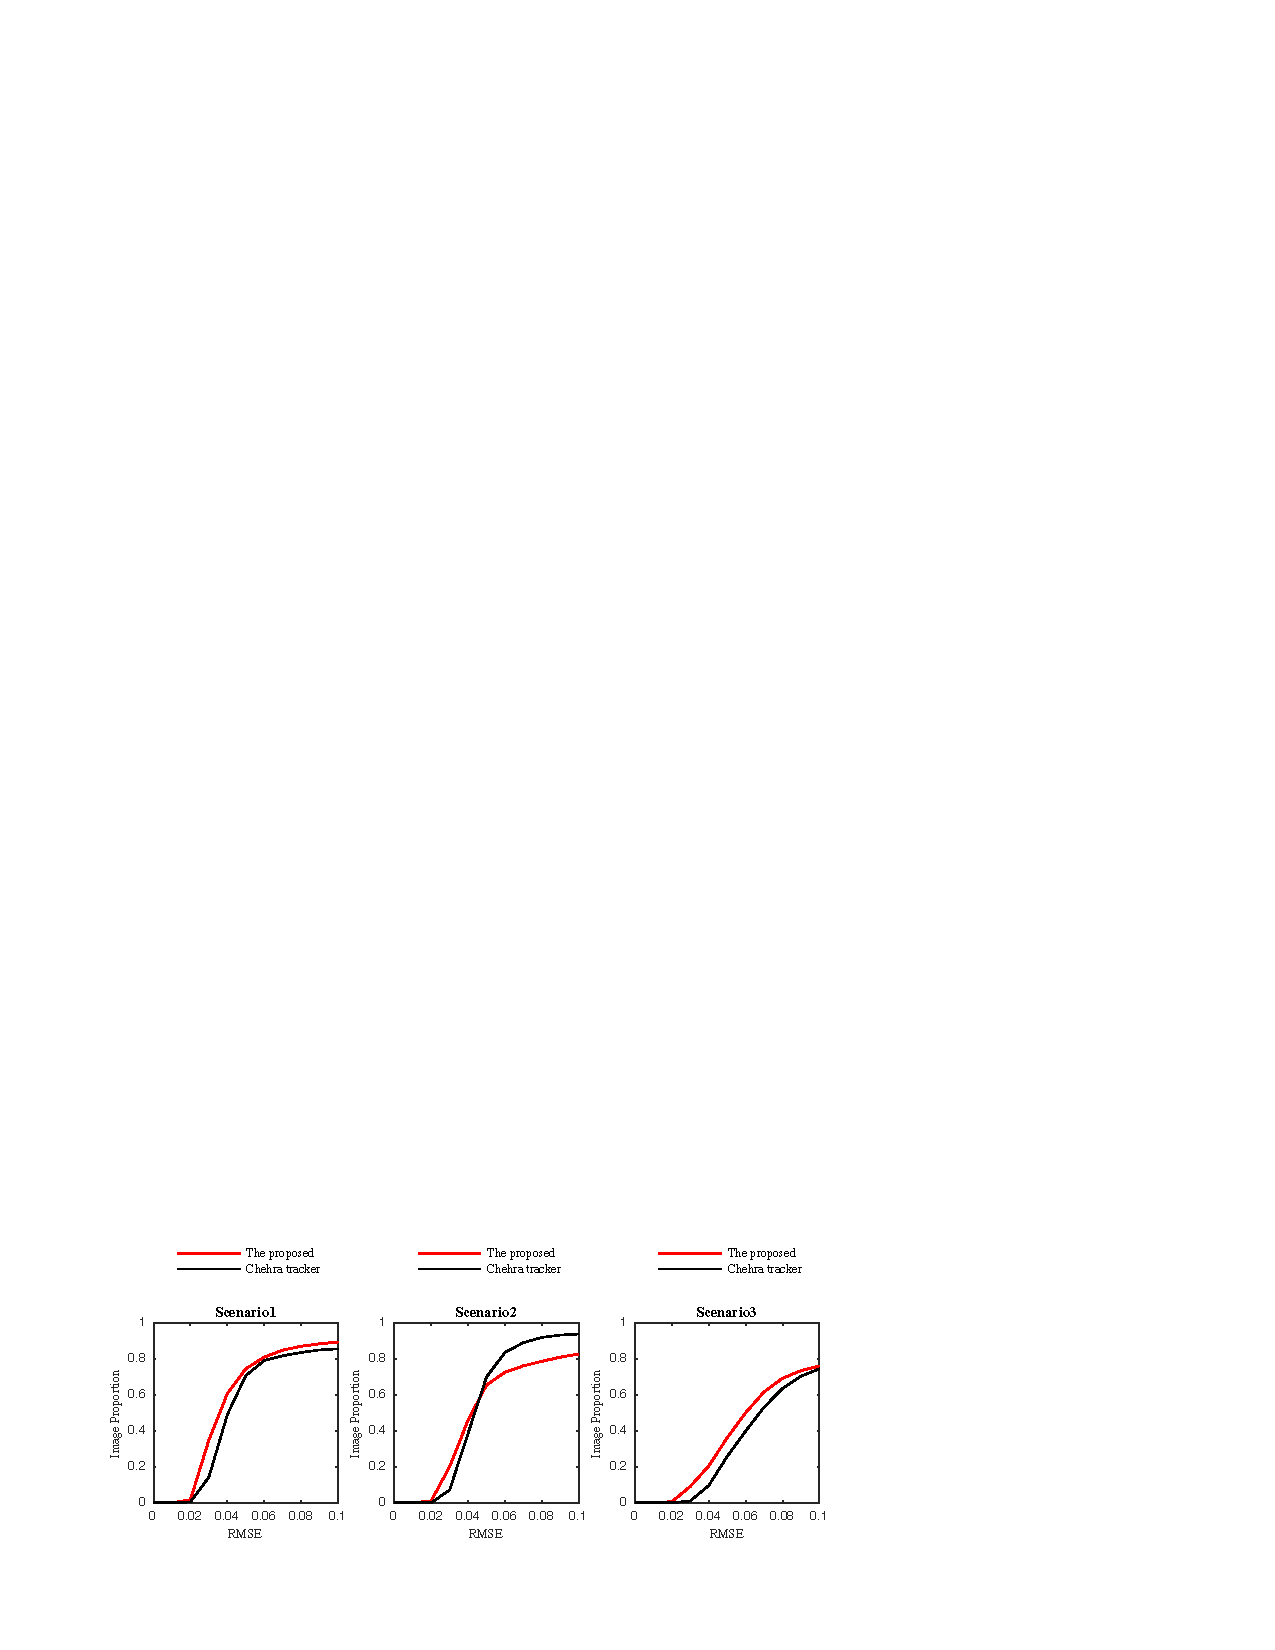
\includegraphics[width=\textwidth,height=0.3\textheight]{Figures_NMSE_img_proportion.pdf}% 1\linewidth  
        \caption{
        Cumulative error curve of the proposed method (red) and the Chehra tracker (black) on 300-VW dataset (49 landmarks).
        The overview of delivery system.
        }
        \label{fig:nmse1}  

        \centering
        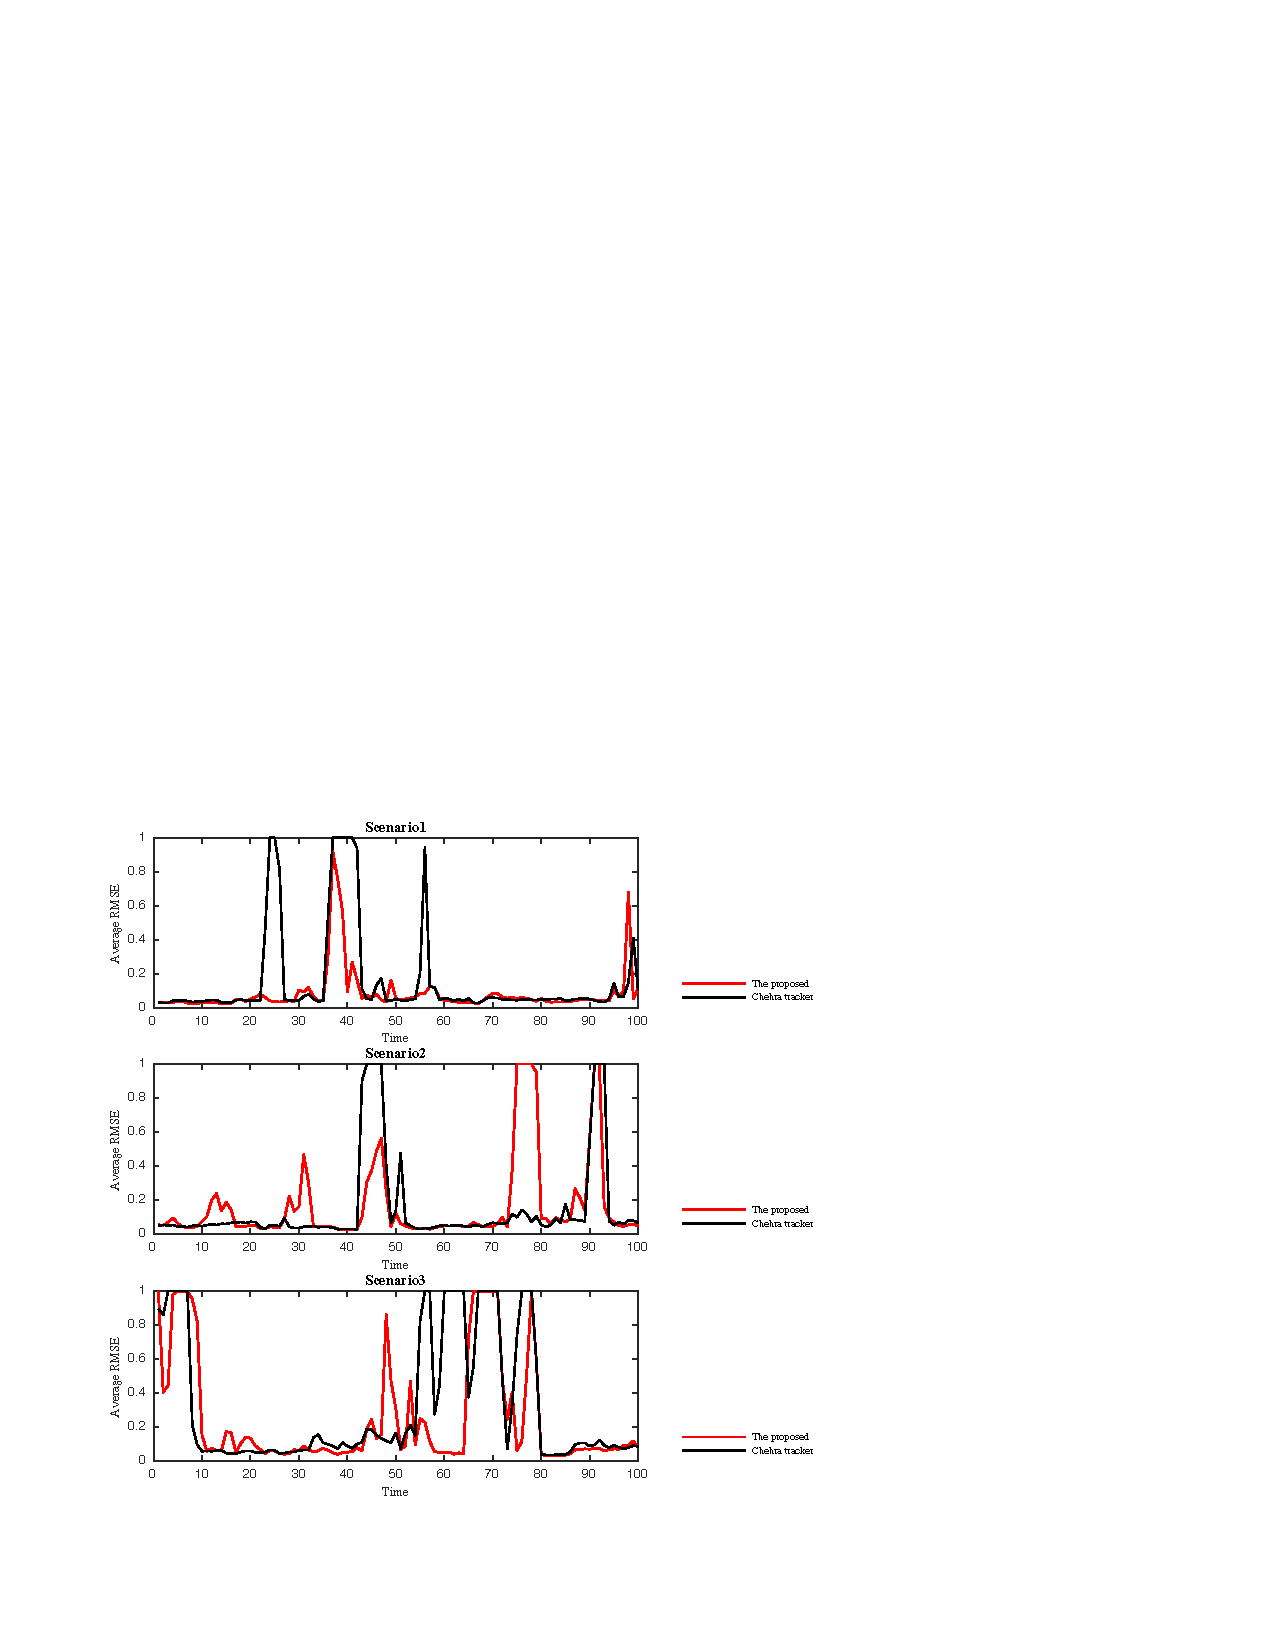
\includegraphics[width=\textwidth,height=0.6\textheight]{Figures_3Secnatios.pdf}
        \caption{
        The frame-by-frame average RMSE plot for proposed method (red) and the Chehra tracker (black) on 300-VW dataset(49 landmarks).
        }
        \label{fig:nmse2}  
\end{figure*}
\begin{figure*}[htbp]
      % Requires \usepackage{graphicx}  
        \centering  
        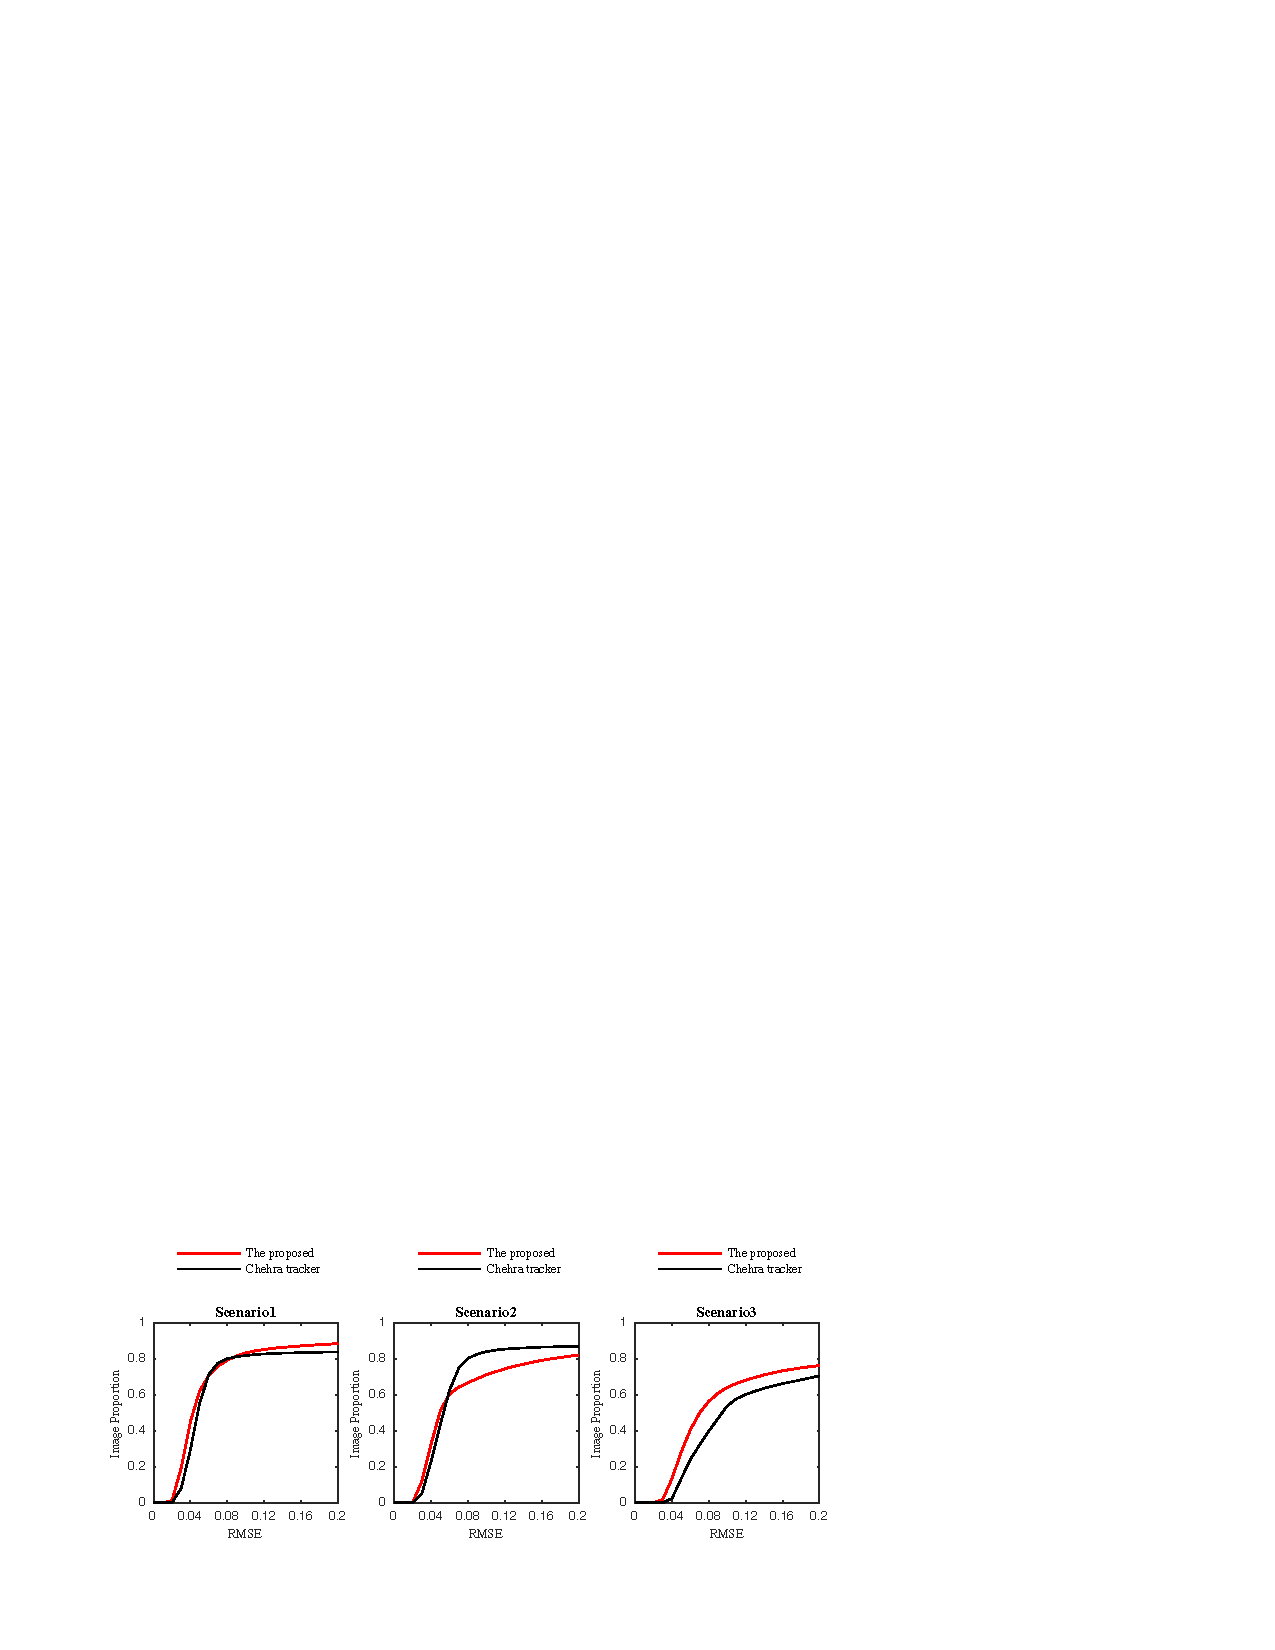
\includegraphics[width=\textwidth,height=0.3\textheight]{Figures_NMSE_img_proportion2.pdf}% 1\linewidth  
        \caption{
        Cumulative error curve of the proposed method (red) and the Chehra tracker (black) on image scale changed 300-VW dataset (49 landmarks).
        The overview of delivery system.
        }
        \label{fig:nmse3}  

        \centering
        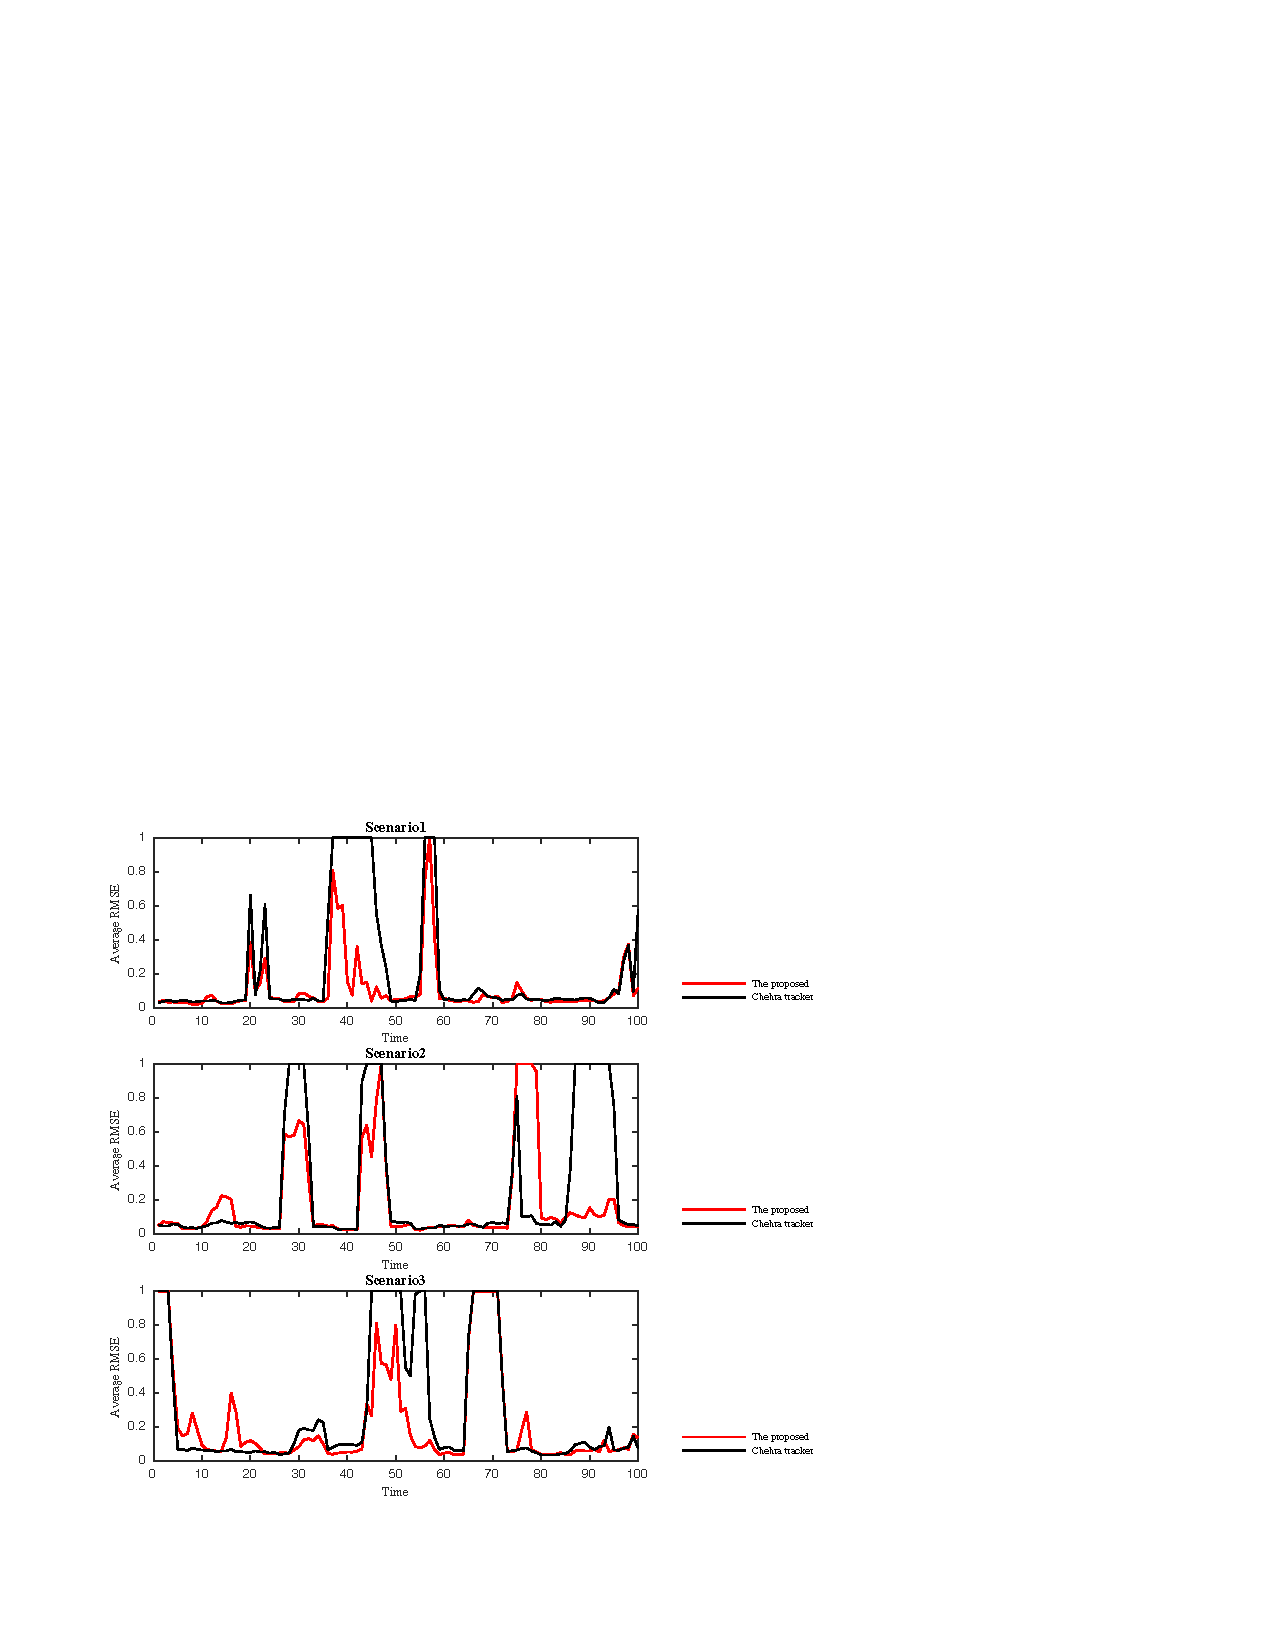
\includegraphics[width=\textwidth,height=0.6\textheight]{Figures_3Secnatios2.pdf}
        \caption{
        The frame-by-frame average RMSE plot for proposed method (red) and the Chehra tracker (black) on image scale changed 300-VW dataset(49 landmarks).
        }
        \label{fig:nmse4}
\end{figure*}
%offline model fitting
\subsection{Fitting Facial Shape Utilizing Trained CS-OFDM}
Our real-time fitting utilizing trained CS-OFDM is performed as illustrated in Figure \ref{fig:fitting}.
Because our approach fits current frame shape by recovering the shape residuals with last frame shape, the fitting of the first frame will be performed
utilizing the mean shape of the annotated shapes. During acquisition, face image can be captured by camera in a real time manner. 
Then the facial shape of each current frame is fitted by the recovery to the shape residuals utilizing the trained CS-OFDM.
To alleviate model drifting, we use the result of the face detection to judge the fitting result. If drift occurs, reboot is performed from mean shape.
\section{Experiments}
In this section we present qualitative and quantitative results on publicly available databases for the novel real-time face alignment 
approach presented in this paper, which serve to demonstrate the accurancy, the smoothness and the real-time performance of the proposed approach. 
We first presents the implementation details about training and experimental settings used in our experiments. Then we describe the publicly video
datasets and evaluation protocols. We compare the proposed approach with the existing state-of-the-art tracking method on the discussed datasets. 
\subsection{Implementation Details}
During the training process, we use image dataset to train our offline model. To simulate the video situation, Each image is regarded as 
current frame, and the last facial shapes are synthesized according to each truly shape corresponding to the current frame. 
Because our offline model recoveries current frame shape by reconstructing the shape residuals with the previous one. The capability that our 
offline model senses the various previous priors can ensure a reliable recovery. Therefore, we sample multiple last facial shapes using a Gaussian 
random pattern around the current truth shape. In our experiment, we generate 20 candidatets for each last facial shape. Once the training 
set is constructed, we train 5000 regression trees by evaluating 500 splitting candidates at each node and the shrinkage factor used
to combat over-fitting is set to 0.01. The depth of the tree is set to 5.
\subsection{Datasets}
We use data from different datasets of static images to construct our training set which consists of: Helen \cite{le2012interactive},
LFPW \cite{belhumeur2013localizing}.
All training images are annotated with a 68-point configuration defined in 300-W challenge \cite{sagonas2013semi}. We compare our approach 
with increment approaches, Chehra tracker, on the 300VW \cite{shen2015first}. The face videos from the dataset are categorized into “Scenario 1”, 
“Scenario 2” and “Scenario 3”. 
Category 1 contains 31 videos recorded in controlled conditions, namely in laboratory and naturalistic well-lit conditions, 
whereas Category 2 includes 19 videos recorded under severe changes in illumination, namely in real-world human-computer interaction applications. 
Category 3 contains 14 videos captured in totally unconstrained scenarios, namely arbitrary conditions with challenge evaluation. 
All the videos are of a single-person, and have been annotated.

Fitting evaluation in all experiments is performed utilizing normalized Root Mean Square Error (RMSE), is computed for each frame by 
dividing the average point-to-point Euclidean error by the distance between two eye centers.

Our approaches are implemented in C++. All experiments are performed on an Intel 7 core 4 GHz CPU with 16 GB RAM. During detection, we 
use the face detector of OpenCV to detect the bounding box. This face detector is realized by Viola and Jones algorithm which uses 
Haar features and a cascade of classifiers.
\subsection{Comparision}
The fitting results of our proposed method and Chehra tracker on the 3 scenarios are reported using the RMSE evaluation metric. Comparison 
between the proposed method and participant is conducted by two types of curves. The first one is Cumulative Error Distribution curve (CED) 
, as shown in Figures \ref{fig:nmse1} and \ref{fig:nmse3}, which examines the ability of our method to track face images in controlled and unconstrained scenarios. 
The second one plots average RMSE as function of time, as shown in Figures \ref{fig:nmse2} and \ref{fig:nmse4}, which reflects the smoothness of tracking results from the two 
participants. In particular, we randomly sample a faction of frames, one hundred of frames in this paper, in all videos of each scenario. Then, 
we average all the RMSE at the same time. At last, we analyze the real-time performance.
\subsubsection{Evaluation on 3 scenarios}
Comparison is performed on three described scenarios, as shown in Figure \ref{fig:nmse1}. Compared to the participant, incremental method,
the performance of the proposed method is much better on two of
the three test sets, namely scenario 1 and scenario 2, as shown in Figure \ref{fig:nmse1}(a and c). 
which indicates that the proposed approach is robust under controlled conditions and arbitrary conditions.
However, our approach does not show a better performance, as shown in Figure \ref{fig:nmse1}(b). One possible reason of this problem is
that videos in 
scenario 2 are recorded under severe changes in illumination and the image feature, difference of two intensities, used by the proposed approach is 
not robust to the severe changes in illumination. Figure \ref{fig:nmse2} shows three average RMSE curves on all scenarios. It can be seen that the proposed approach
has a smaller average RMSE on scenario 1 and 2 at nearly the beginning and end of tracking, and shows a more smooth fitting results.
Otherwise, the participant method exhibits more severe phenomenon. As discussed, our proposed approach does not provide a better fitting under the 
condition with severe changes in illumination. In summary, Our proposed approach provides a robust performance under many conditions expect the 
illumination.
\subsubsection{Robust evaluation}
In order to evaluate the comparison under severe changes in the size of image, each image in all scenarios is normalize into the size of 
640$\times$480, 
in which 640 represents the width of a image, and 480 is the height. From the other viewpoint, it also simulates the smart-phone environment. We 
achieve all the ground truth shapes by applying Procrustes Analysis to the original ground truth ones. Figures \ref{fig:nmse3} and \ref{fig:nmse4}
show nearly same results as that in Figures \ref{fig:nmse1} and \ref{fig:nmse2}. Moreover, our proposed method provide more robust results in scenario 2.
Therefore, our proposed approach is robust to the changes in the size of image, and is more suitable to the smart-phone.
\subsubsection{Analysis of real-time performance}
The real-time performance of our proposed approach is similar to that of regression tree based static face alignment approaches for there similarity
in efficiency of alignment to face shape. At the same time, the regression tree based static face alignment approaches are certificated to be of
super real-time performance. Therefore, our approach can provide a better real-time performance than the existing state-of-the-art incremental
learning based ones and achieves over 166 fps on a desktop.
%Finally, we compare the real-time performance on the existing state-of-the-art methods in table I. From the table, we can know that our proposed 
%method is the fastest method, namely a super real-time method.
\section{Conclusion}
In this paper, we investigate the problem of smooth and accurate landmark-detection for real-time face alignment. We propose a novel compressive 
sensing based offline FDM for smoothly detect the location of the facial landmarks by recovering the shape residuals between consequent frames. 
Our trained offline model is composed of separate discriminative tree based sparse transforms, which are directly learned from samples of the 
facial shape residuals between the ground truth facial shape of the current frame and simulated facial shapes of last frame, which are randomly 
sampled around the current facial shape. Furthermore, we propose a strategy to oppose the drift during tracking. This allows our approach to keep 
a long period of tracking. We conduct experiments on the 300-VW challenge datasets. The results clearly demonstrate that our approach provides 
significant improvement over the baseline on the smooth performance.
% We also compare our approach with several state-of-the-art methods on the 
% real-time performance. The result indicates that our proposed method is super real-time.
We also analysis the real-time performance of our approach. 
However, the intensity difference based image feature is 
not robust to the illumination changes.
Therefore, We plan to investigate efficient feature fusion strategies to combine intensity and color information.
Another research direction is to investigate more accurate sparse transform to produce better sparse approximation.
%\par
%\centerline{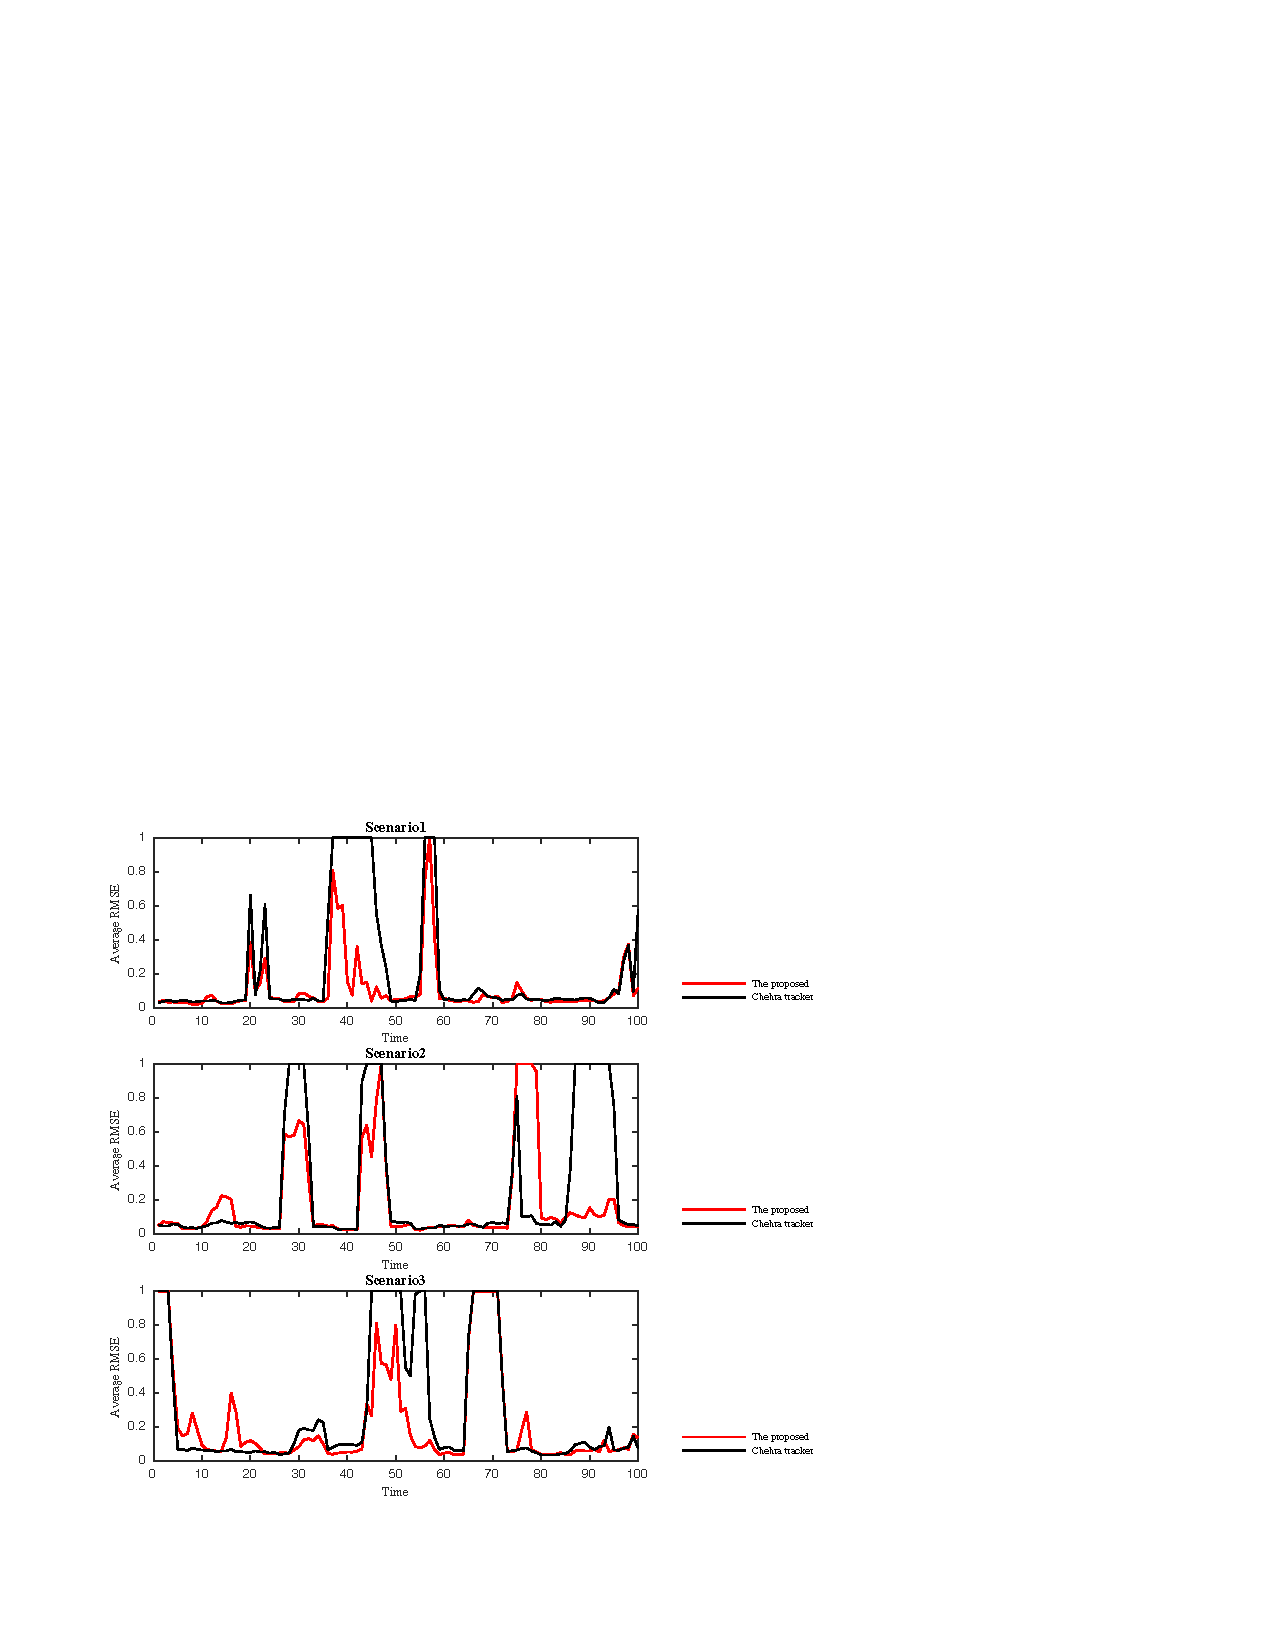
\includegraphics[height=6cm,width=12cm]{Figures_3Secnatios2.pdf}} 
%\centerline{Figure 1 This is lena}
%\par
\begin{comment}
\begin{table}
\caption{An Example of a Table}
\label{table_example}
\begin{center}
\begin{tabular}{|c||c|}
\hline
One & Two\\
\hline
Three & Four\\
\hline
\end{tabular}
\end{center}
\end{table}
\end{comment}

%conference
\bibliographystyle{ieeetr}
\bibliography{conference.bib}

\end{document}
